\documentclass[12pt, a4paper]{article}
% !TEX program = xelatex
\usepackage{mbi6013}

\begin{document}

% ==========================================
% Title Page
% ==========================================
\begin{titlepage}
    \centering
    \vspace*{2cm}

    {\LARGE \bfseries Research Proposal: Deciphering Single-Cell Multi-Omic and Genetic Regulatory Programs of Pathogenic B-Cell States in Systemic Lupus Erythematosus\par}
    
    \vspace{2.5cm}
    
    {\Large \textbf{Student ID:} 225050069\par}
    \vspace{0.5cm}
    {\Large \textbf{Student Name:} Chen Zhi\par}
    \vspace{0.5cm}
    {\Large \textbf{Mentor:} Prof. Yongfei Wang\par}
    \vspace{0.5cm}
    {\Large \textbf{Course Instructor:} Prof. Yongfei Wang\par}
    \vspace{0.5cm}
    {\Large \textbf{Department:} Graduate Program in Bioinformatics\par}
    \vspace{0.5cm}
    {\Large \textbf{Institution:} The Chinese University of Hong Kong, Shenzhen\par}
    
    \vfill
    
    {\large April 2026\par}
\end{titlepage}

\newpage

% ==========================================
% A. Background and Significance
% ==========================================
\section*{A. Background and Significance}
\addcontentsline{toc}{section}{A. Background and Significance}

Systemic lupus erythematosus (SLE) is a heterogeneous autoimmune disease with marked variation in clinical manifestations, molecular activity, and treatment response. Although type I interferon signaling, autoantibody production, and lymphocyte dysregulation are recognized as central hallmarks of SLE, these features alone do not fully explain why patients differ so substantially in disease severity, tissue involvement, and therapeutic response. Bulk transcriptomic approaches and conventional marker-based immune phenotyping have provided important insights, but they are limited in their ability to resolve disease-relevant immune states at cellular resolution. Recent advances in single-cell technologies have therefore become especially important in lupus research because they enable simultaneous dissection of altered immune-cell abundance, cell-state remodeling, and context-dependent molecular programs.

Among the immune compartments implicated in lupus pathogenesis, B cells are particularly important because they integrate several layers of disease biology at once. They can differentiate into antibody-secreting cells, present antigen to T cells, respond to innate nucleic-acid sensing pathways, and participate in inflammatory amplification loops. Increasing evidence suggests that lupus-associated B-cell pathology is not driven by a single abnormal subset, but by a continuum of pathogenic states that includes age-associated B cells (ABCs), DN2-like cells, activated memory-like B cells, plasmablast-associated states, and antigen-presenting B-cell states. A state-based framework is therefore more informative than a simple subset-counting model for understanding lupus B-cell biology.

This conceptual shift is strongly supported by recent studies. Perez et al.\ profiled more than 1.2 million peripheral blood mononuclear cells from SLE cases and controls and showed that lupus is associated not only with altered immune composition but also with cell type--specific transcriptional programs and cell type--specific cis-expression quantitative trait loci (cis-eQTLs) \cite{Perez2022}. Dai et al.\ demonstrated that the transcription factor ZEB2 is required for human and mouse ABC differentiation and is essential for ABC accumulation in lupus-related settings, establishing ZEB2 as a functional driver rather than a passive marker of pathogenic B-cell fate \cite{Dai2024}. Zeng et al.\ further linked TLR7--MyD88 signaling to ABC differentiation through the m\textsuperscript{6}A demethylase FTO and its downstream target ATP6V1G1, connecting innate sensing, epitranscriptomic regulation, lysosomal function, mitochondrial oxidative metabolism, and pathogenic B-cell expansion \cite{Zeng2025}. In parallel, Younis et al.\ showed that Epstein--Barr virus (EBV)-positive B cells in SLE are predominantly CD27\textsuperscript{+}CD21\textsuperscript{low} memory B cells with antigen-presenting-cell-like transcriptional features and upregulation of ZEB2, TBX21, and antigen-presentation pathways \cite{Younis2025}. Together, these studies suggest that apparently distinct lupus B-cell observations may converge on shared regulatory circuits involving innate activation, altered differentiation, and inflammatory cell-state remodeling.

A major unresolved challenge is how to connect lupus-focused disease studies with broader immune regulatory architecture. Population-scale immune genetic resources now offer a powerful opportunity to address this problem. The OneK1K study generated single-cell RNA-seq data from 1.27 million peripheral blood mononuclear cells across 982 donors and showed that many genetic effects on gene expression are highly cell type--specific, including dynamic eQTL effects along the B-cell maturation landscape from naive to memory states \cite{Yazar2022}. More recently, the Chinese Immune Multi-Omics Atlas (CIMA) profiled more than 10 million immune cells from 428 Chinese adults using scRNA-seq and scATAC-seq, constructed enhancer-driven gene regulatory networks, mapped cell type--resolved eQTLs and caQTLs, and detected dynamic eQTL effects in B cells \cite{Yin2026}. These resources make it possible to ask not only which genes mark pathogenic lupus B-cell states, but also which regulators and loci are most plausibly linked to those states in the broader human immune system.

At the same time, lupus biology cannot be reduced to blood alone. Tissue-context studies indicate that inflammatory programs vary across disease sites and clinical phenotypes. Zheng et al.\ reported pronounced cellular heterogeneity and enhanced intercellular communication in cutaneous lesions of lupus erythematosus \cite{Zheng2022}. Lee et al.\ further showed that distinct cutaneous manifestations of SLE are associated with different transcriptomic and pathway signatures, including differential enrichment of interferon, TNF-$\alpha$, and IL6--JAK--STAT3 programs \cite{Lee2025}. These observations reinforce the need to interpret circulating B-cell signatures within a broader disease-context framework rather than assuming that all lupus-relevant programs are universal across tissues.

Taken together, the current literature supports a central idea: lupus pathogenicity is mediated not simply by the abundance of broad immune lineages, but by disease-relevant cellular states embedded within regulatory, genetic, and inflammatory contexts. A systematic integrative analysis focused on lupus B-cell states is therefore both timely and biologically significant.

% ==========================================
% B. Specific Aims
% ==========================================
\section*{B. Specific Aims}
\addcontentsline{toc}{section}{B. Specific Aims}

The long-term objective of this research is to clarify how pathogenic B-cell states arise and are regulated in systemic lupus erythematosus. The central hypothesis is that pathogenic lupus B-cell states form a partially connected continuum and that their most meaningful candidate drivers can be prioritized by convergence across four evidence layers: state specificity, trajectory relevance, external immune regulatory support, and disease-focused mechanistic plausibility. To test this hypothesis, I propose the following specific aims:

\begin{itemize}[leftmargin=*]
    \item \textbf{Aim 1: Construct a high-resolution atlas of pathogenic B-cell states in SLE.} I will assemble and harmonize public lupus single-cell datasets, perform quality control and integration, and re-cluster the B-cell compartment to define ABC/DN2-like, activated memory-like, plasmablast-associated, and antigen-presenting B-cell states.
    
    \item \textbf{Aim 2: Define the transition logic and inflammatory embedding of pathogenic B-cell states.} I will infer trajectory relationships among prioritized B-cell states, quantify pathway activity, and examine the intercellular environments in which these states are embedded, with particular attention to innate sensing, interferon-associated signaling, antigen presentation, and T--B or myeloid--B interactions.
    
    \item \textbf{Aim 3: Prioritize candidate regulators and genetically supported mechanisms of pathogenic B-cell states.} I will integrate lupus B-cell state signatures with external immune genetic and multi-omic resources, especially OneK1K and CIMA, to identify overlapping dynamic eQTLs, regulatory modules, and biologically plausible drivers such as ZEB2-, TBX21-, and FTO-related programs.
\end{itemize}

Successful completion of these aims will generate a mechanism-oriented map of lupus B-cell states and produce an evidence-ranked shortlist of candidate regulators for future validation.

% ==========================================
% C. Preliminary Data
% ==========================================
\section*{C. Preliminary Data}
\addcontentsline{toc}{section}{C. Preliminary Data}

At this stage, the proposed work is designed as a computationally tractable, literature-anchored, and data-driven project based primarily on publicly available datasets. Although no new wet-lab data have yet been generated specifically for this proposal, several lines of published evidence strongly support the feasibility of the project.

First, large-scale lupus single-cell datasets already demonstrate that disease-associated immune states can be resolved at high resolution in peripheral blood. Perez et al.\ showed that SLE is associated with altered immune-cell composition, state-specific transcriptional programs, and cell type--specific genetic associations in peripheral blood mononuclear cells \cite{Perez2022}. These findings provide direct support for the feasibility of a state-focused analysis framework in lupus.

Second, disease-focused mechanistic studies provide concrete candidate programs that can be explicitly tested in an integrative framework. Dai et al.\ established ZEB2 as a key regulator of ABC formation \cite{Dai2024}; Zeng et al.\ linked TLR7-driven ABC differentiation to FTO-dependent metabolic and lysosomal regulation \cite{Zeng2025}; and Younis et al.\ identified EBV-associated APC-like autoreactive B-cell reprogramming in SLE \cite{Younis2025}. These studies provide strong biological anchors for prioritizing candidate regulators in the proposed analysis.

Third, the external immune regulatory resources required for systematic prioritization already exist in population-scale form. OneK1K provides dynamic B-cell eQTL information across the naive-to-memory axis \cite{Yazar2022}, and CIMA extends this framework through integrated scRNA-seq, scATAC-seq, gene regulatory networks, and xQTL mapping in a large Chinese population cohort \cite{Yin2026}. These resources make it realistic to move beyond descriptive clustering and toward mechanism-oriented prioritization.

Finally, the current working draft of this proposal has already established a coherent biological question, a B-cell-state-centered scope, and a feasible computational roadmap. The present version therefore builds on an existing conceptual and organizational foundation, rather than starting from an unstructured exploratory idea.

% ==========================================
% D. Research (Experimental) Design and Methods
% ==========================================
\section*{D. Research (Experimental) Design and Methods}
\addcontentsline{toc}{section}{D. Research Design and Methods}

\subsection*{D.1 Underlying Methodology and Rationale}

\subsubsection*{Overview}
This project will adopt a multi-stage computational strategy integrating lupus single-cell transcriptomic datasets with immune genetic and multi-omic reference resources. The overall workflow consists of four major components: dataset assembly and harmonization, high-resolution B-cell state annotation, trajectory and inflammatory-context analysis, and integrative regulatory prioritization.

\subsubsection*{Rationale}
The methodological rationale is based on the idea that pathogenic lupus B-cell states should not be interpreted solely through differential gene expression within a single dataset. Instead, robust biological prioritization requires convergence across state specificity, dynamic behavior, external regulatory support, and disease-focused plausibility. This design is especially appropriate for lupus, where disease heterogeneity, tissue context, and immune-state plasticity complicate simple subset-based explanations.

\subsubsection*{Key Methods}
Public lupus single-cell datasets relevant to peripheral blood and selected tissue contexts will be collected and harmonized using standardized metadata. After quality control, normalization, and study-aware integration, the B-cell compartment will be extracted and re-clustered at higher resolution. Candidate states will be annotated using canonical markers and disease-informed interpretation from the literature, focusing on ABC/DN2-like cells, activated memory-like cells, plasmablast-associated states, and antigen-presenting B-cell states.

Differential-state characterization will include marker analysis, pathway enrichment, and program-level scoring, with emphasis on interferon signaling, innate sensing, antigen presentation, and metabolic remodeling. Trajectory or pseudotime analyses will then be used to infer how prioritized B-cell states are related, including whether they behave as connected differentiation trajectories or relatively distinct inflammatory endpoints.

To place these states into their inflammatory environments, I will perform intercellular communication analysis between prioritized B-cell states and other immune or tissue compartments when relevant. Particular attention will be given to interactions involving T cells, myeloid cells, and antigen-presentation-associated signaling.

Finally, state-specific lupus signatures will be integrated with OneK1K and CIMA to identify overlapping dynamic eQTLs, eGenes, caPeaks, and regulatory modules. Candidate drivers will be ranked using an evidence-convergence framework that combines lupus state specificity, trajectory relevance, external immune regulatory support, and disease-focused mechanistic plausibility.

\textbf{Optional figure placeholder:} The figure below can be replaced by a project-specific workflow diagram summarizing data collection, B-cell re-clustering, trajectory inference, and regulatory prioritization.

\begin{figure}[H]
    \centering
    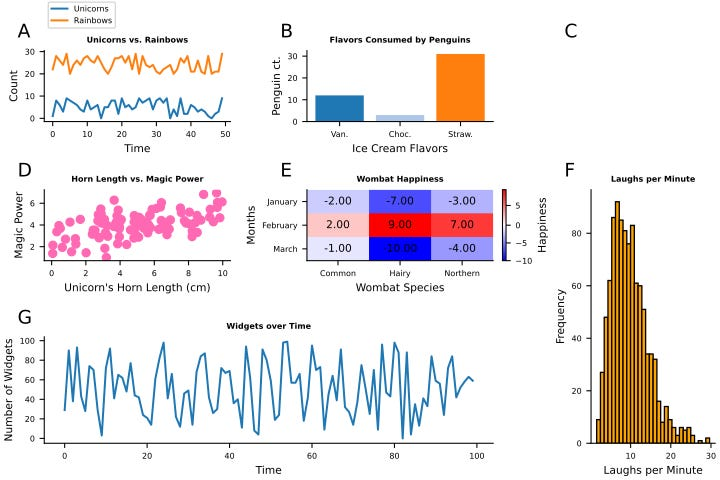
\includegraphics[width=0.85\textwidth]{assets/example.png}
    \caption{Placeholder for a study workflow figure. In the final version, this panel can be replaced with a schematic showing dataset assembly, B-cell state annotation, trajectory analysis, and integration with immune genetic and multi-omic resources.}
    \label{fig:workflow}
\end{figure}

\subsection*{D.2 Data Analysis and Interpretation}

Data analysis will primarily be conducted in R and Python using standard single-cell and statistical analysis frameworks. Depending on dataset format and compatibility, preprocessing and integration may involve Seurat, Scanpy, or related tools. Pathway analysis will be performed using established enrichment approaches, and communication analysis will be implemented using ligand--receptor inference methods suitable for the available datasets.

Whenever donor-level information is available, donor-aware models or pseudobulk strategies will be preferred over naive cell-level testing. Multiple-testing correction will be applied using false discovery rate control. For trajectory analysis, results will be interpreted cautiously as models of state relationships rather than direct proof of lineage commitment. For communication analysis, ligand--receptor signals will be treated as contextual hypotheses rather than definitive evidence of causal cell--cell interaction.

The interpretation of final results will be guided by the central hypothesis and the three specific aims. In particular, the final emphasis will not be on producing a long list of differentially expressed genes, but on generating a ranked shortlist of candidate regulators and mechanistic programs that are supported across multiple evidence layers.

\subsection*{D.3 Potential Difficulties and Alternative Approaches}

One major challenge is dataset heterogeneity. Lupus single-cell datasets differ in cohort composition, sequencing chemistry, tissue source, sample size, and annotation depth. If cross-dataset integration obscures biologically meaningful rare states, I will complement integrated analyses with study-specific analyses and focus on robust state signatures rather than forcing exact cluster matching across studies.

A second limitation is that external immune genetic resources such as OneK1K and CIMA are not lupus-specific. Therefore, overlap with these resources will be interpreted as prioritization evidence rather than definitive proof of lupus-specific causality. To address this issue, I will require convergence across multiple evidence layers before assigning high priority to any candidate regulator.

A third challenge is that blood-derived signatures may not generalize to tissue disease. Rather than assuming universal transferability, I will use selected cutaneous lupus resources as a contextual validation layer. Failure to replicate a blood-derived signature in tissue will be interpreted cautiously and may reflect phenotype restriction or compartment specificity rather than absence of biological relevance.

Finally, full perturbational validation is beyond the scope of the current project. Accordingly, this proposal is explicitly framed as a mechanism-prioritization study that will generate testable hypotheses for future experimental follow-up.

\subsection*{D.4 Timetable}
\begin{itemize}
    \item \textbf{Months 1--2:} Dataset collection, metadata harmonization, and establishment of a reproducible analysis environment.
    \item \textbf{Months 3--4:} Quality control, normalization, integration, B-cell extraction, and high-resolution re-clustering.
    \item \textbf{Months 5--6:} Differential-state characterization, pathway analysis, and trajectory inference.
    \item \textbf{Months 7--8:} Intercellular communication analysis and inflammatory-context characterization.
    \item \textbf{Months 9--10:} Integration with OneK1K and CIMA; regulatory and genetic prioritization of candidate drivers.
    \item \textbf{Months 11--12:} External contextualization, final interpretation, figure preparation, and writing.
\end{itemize}

% ==========================================
% E. Bibliography or Reference List
% ==========================================
\newpage
\section*{E. Bibliography or Reference List}
\addcontentsline{toc}{section}{E. Bibliography}

\begin{thebibliography}{99}

\bibitem{Perez2022}
Perez RK, Gordon MG, Subramaniam M, et al.
Single-cell RNA-seq reveals cell type-specific molecular and genetic associations to lupus.
\textit{Science}. 2022;376:eabf1970.

\bibitem{Dai2024}
Dai D, Gu S, Han X, et al.
The transcription factor ZEB2 drives the formation of age-associated B cells.
\textit{Science}. 2024;383:413--421.

\bibitem{Zeng2025}
Zeng Q, Li L, Li X, et al.
The m\textsuperscript{6}A demethylase FTO links TLR7 to mitochondrial oxidation driving age-associated B cell formation in systemic lupus erythematosus.
\textit{Science Translational Medicine}. 2025;17:eadu6015.

\bibitem{Younis2025}
Younis S, Moutusy SI, Rasouli S, et al.
Epstein--Barr virus reprograms autoreactive B cells as antigen-presenting cells in systemic lupus erythematosus.
\textit{Science Translational Medicine}. 2025;17:eady0210.

\bibitem{Yazar2022}
Yazar S, Alquicira-Hernandez J, Wing K, et al.
Single-cell eQTL mapping identifies cell type-specific genetic control of autoimmune disease.
\textit{Science}. 2022;376:eabf3041.

\bibitem{Yin2026}
Yin J, Zheng Y, Huang Z, et al.
Chinese Immune Multi-Omics Atlas.
\textit{Science}. 2026;391:eadt3130.

\bibitem{Zheng2022}
Zheng M, Hu Z, Mei X, et al.
Single-cell sequencing shows cellular heterogeneity of cutaneous lesions in lupus erythematosus.
\textit{Nature Communications}. 2022;13:7489.

\bibitem{Lee2025}
Lee EY, Patterson S, Cutts Z, et al.
Transcriptomic analysis reveals immune signatures associated with specific cutaneous manifestations of lupus in systemic lupus erythematosus.
\textit{bioRxiv}. 2025.

\end{thebibliography}

\end{document}